


Flavour physics could be instrumental in searches for dark matter or dark sectors. Light dark sector particles can be produced in \textbf{flavour violating rare decays}, for instance in $B\to K X_{\rm dark}$, $B\to D X_{\rm dark}$, $D\to K X_{\rm dark}$, $K\to \pi X_{\rm dark}$, either through tree level or one loop mediated emissions of dark sector particles, see, e.g., Refs.~\cite{Bird:2004ts,Kamenik:2011vy}. Such decays are an exciting and increasingly important drivers in the searches for dark sector candidates, since they are often the dominant production channels. Particles that 
either carry nonzero flavour or have flavour violating couplings  may  thus be produced in the flavour violating transitions at tree level, as for instance, heavy neutral leptons \cite{Gorbunov:2007ak} and the  axiflavon~\cite{Calibbi:2016hwq,Ema:2016ops,Wilczek:1982rv}. 
Examples of particles with flavour diagonal couplings, produced in meson decays induced at one loop via $W^\pm$ exchange, include a light singlet scalar mixing with the Higgs~\cite{OConnell:2006rsp,Batell:2009jf,Winkler:2018qyg},  ALPs (axion-like particles)~\cite{Jaeckel:2010ni}, and some dark matter candidates. It is  interesting that even the experiments whose primary goals are in flavour physics, such as NA62 or the Upgrade II of LHCb, have significant discovery potential in dark sector searches. 

The dark sector particles in the final state, $X_{\rm dark}$, may decay back into visible particles and be detected or, alternatively, result in missing energy and momentum, if they are sufficiently long-lived
or decay to neutrinos. 
When visible, the vertex may be prompt or displaced, depending on the lifetime of $X_{\rm dark}$.   There are a number of proposed experiments, with a clear synergy between different search strategies, such as searches for displaced vertices, monojets, etc. In the {\bf short-term}  the existing and approved experiments, Faser~\cite{Feng:2017uoz}, NA62~\cite{Gonnella:2017hsz}, NA64~\cite{Banerjee:2016tad}, SeaQuest~\cite{Berlin:2018pwi}, LHCb, ATLAS and CMS could explore different dark sector models. In the {\bf mid-term} the proposed experiments, such as beam dump mode of NA62~\cite{Beacham:2019nyx}, LHCb combined with Codex-b~\cite{Gligorov:2017nwh}, Belle II combined with Gazelle, LDMX~\cite{Akesson:2018vlm}, Mathusla~\cite{Chou:2016lxi,Alpigiani:2018fgd}, and SHiP~\cite{Alekhin:2015byh}   could explore large regions of presently unconstrained parameter space, see Fig.~\ref{fig:dark:daulepton} for two examples. 
  Also in the mid-term, Upgrade II of LHCb will have improved sensitivity to dark photons from $D^*\to D\gamma_{\rm dark}$ decays or from bump hunting in the $\mu^+\mu^-$ spectra. In the {\bf long-term}  \FCCee  could significantly increase the reach for dark sector masses, e.g. to a further order of magnitude in mass. 

The  sensitivity of the proposed experiments  to {\bf heavy neutral leptons} mixing with active neutrino flavours is discussed in Sect.~\ref{hnl-sec-nu}.  The  reach for the case in which they mix predominantly with the electron or with the tau flavour, as well as the present bounds (shaded regions), are  illustrated in Fig.~\ref{fig:FIPs-HNL} and  Fig.~\ref{fig:dark:daulepton} (upper panel), respectively.  There is clearly a very strong potential for a whole suite of experiments. 
%Similarly is true of 
The same holds for other sample models, for instance for a {\bf Higgs-mixed singlet scalar} $S$, shown in Fig.~\ref{fig:dark:daulepton} (lower panel). While smaller scale experiments such as NA62++, FASER and CODEX-b can cover substantial parts of the parameter space for light new dark sectors, the two
 experiments proposed in this regime
  with larger (and comparable) reach in many models  
 are MATHUSLA and SHiP. MATHUSLA and CODEX-b can also probe dark sector particles with masses above few GeV if they originate from decays of heavier states, such as $h\to SS$ decays as illustrated in  Fig.~\ref{fig:dark:daulepton} (lower panel). Overall, the combination of LHCb Upgrade II and CODEX-b, and of ATLAS/CMS and MATHUSLA would cover a very diverse and wide range of new physics options. Heavier dark sectors can be probed in the long-term at \FCCee and/or \CEPC relying on their expected large numbers of $Z$ decays. 


\begin{figure}[t]
	\centering 
	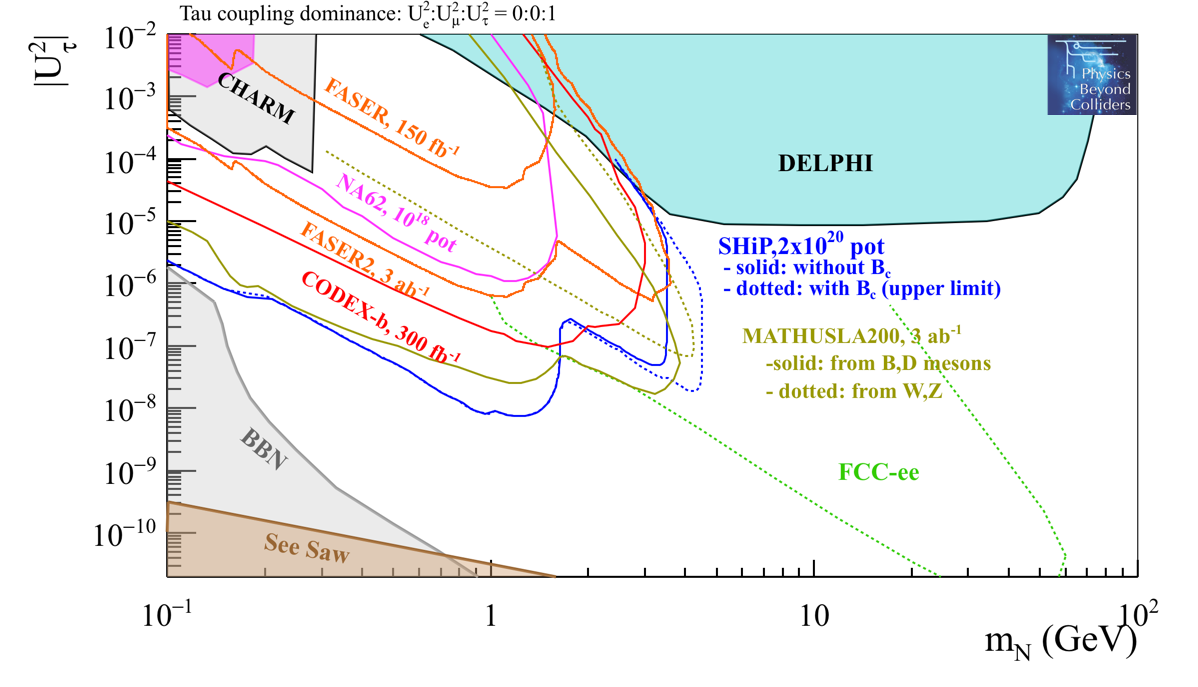
\includegraphics[width=0.8\textwidth]{\main/Flavour/figs/HNL_bc8_pbc_2.png}\\
	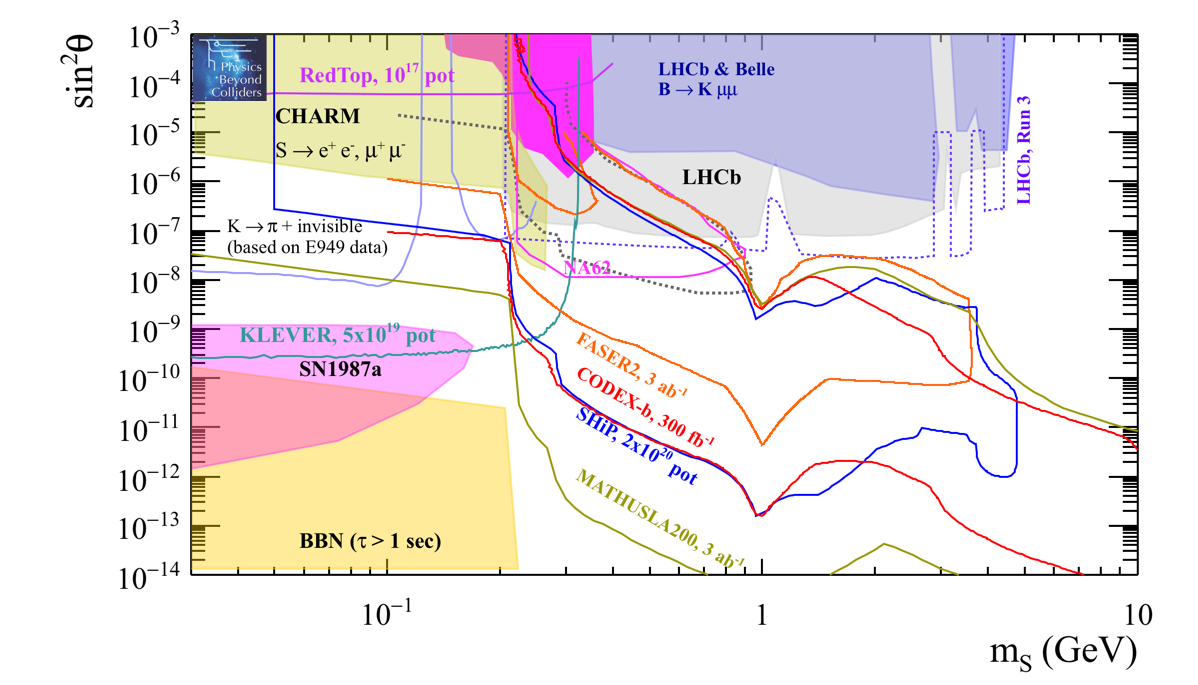
\includegraphics[width=0.8\textwidth]{\main/Flavour/figs/BC5_pbc_2.png}
	\caption{Reach of proposed experiments for heavy neutral leptons coupling predominantly to the tau flavour (top panel) and for Higgs-mixed scalar (bottom panel). From Ref.\cite{Beacham:2019nyx}.	
	\label{fig:dark:daulepton}}
\end{figure}

There is also sensitivity to dark sector mediators in \textbf{classical flavour observables} such as \textbf{meson mixings},  or \textbf{${(g-2)}$ of the muon}. They can contribute at tree-level, in which case the flavour experiments can probe very high scales for ${\mathcal O}(1)$ couplings, or at loop-level as is the case for some   DM candidates and the accompanying $Z_2$-odd mediators. 

An intriguing possibility is that flavour physics might be directly involved in the structure of the dark sector or in its cosmological consequences. For instance, the stability of dark matter could be due to flavour symmetries; striking examples of cosmological consequences of flavour structures are the option of low-scale ($1-100$ GeV) baryogenesis via heavy neutral leptons~\cite{Akhmedov:1998qx,Asaka:2005pn}, or 
having CP violation solely from the SM sector through meson mixing oscillations, whose signature would be seemingly baryon-violating flavour transitions with missing energy (such as $B\to \Lambda 
X_{\rm dark}$)~\cite{Nelson:2019fln,Elor:2018twp}. 
 Conversely, a better understanding of 
 the SM flavour puzzle could potentially come by studying the flavour structure of dark sector.


